\section{Appendix}
\subsection{Proofs}
Unless stated explicitely, all the propositions consider the Multi-Target linear regression problem.
\begin{proposition}
\label{gps_equivalence}
  $\forall (n, p) \in \mathbb{N}_+^2, \bm{y} \in \mathbb{R}^{n}, \bm{x} \in \mathbb{R}^{p} \lambda \in \mathbb{R}$
  
  \begin{align*}
    & \min_{\bf{A}} \norm{\bf{y} - \bf{A}\bf{x}}_2^2 + \lambda \sum_{j=1}^p \norm{\left(A^T\right)_j}_2 \\
     = &\min_{\bf{A'}, \bm{\beta}} \norm{\bf{y} - \bf{A'}\diag{\bm{\beta}}\bf{x}}_2^2 + \lambda \norm{\bm{\beta}}_1 \\
     & \text{s.t.} \forall j, 1 \leq j \leq p, \norm{\left(A'^T\right)_j}_2^2 = 1
  \end{align*}
\end{proposition}

\begin{proof}
  we will split this proof in two different sections. the first one will
  demonstrate that there is at least one global minimum. and the second
  will show how to construct $2^k$ distinct solutions from a single global
  minimum.
  In order to prove this statement we will show that for any solution $\bm{A}$ in the first problem, there exists a solution in the second with the exact same value, and vice-versa.
  \\ \textbf{Part 1:} We assume we have a potential solution $\bm{A}$ for the first problem and we define $\bm{\beta}$ such that $\bm{\beta}_j = \norm{\left(\bm{A}^T\right)_j}_2^2$, and $\bm{A}' = \bm{A}\left(\diag{\bm{\beta}}\right)^{-1}$. It is easy to see that the constraint on $\bm{A}'$ is statisfied by construction. Now:
  \begin{align*}
    & \norm{\bf{y} - \bf{A}\bf{x}}_2^2 + \lambda \sum_{j=1}^p \norm{\left(A^T\right)_j}_2 \\
    = &\norm{\bf{y} - \bf{A'}\diag{\bm{\beta}}\bf{x}}_2^2 + \lambda \sum_{j=1}^p \norm{\left(A'^T\right)_j\beta_j}_2 \\
    = &\norm{\bf{y} - \bf{A'}\diag{\bm{\beta}}\bf{x}}_2^2 + \lambda \sum_{j=1}^p \abs{\beta_j} \cdot 1\\
    = &\norm{\bf{y} - \bf{A'}\diag{\bm{\beta}}\bf{x}}_2^2 + \lambda \norm{\bm{\beta}}_1
  \end{align*}
  Which concludes the first part.
  \\ \textbf{Part 2:} Assuming we take an $\bm{A}'$ that satisfy the constraint and a $\bm{\beta}$, we can define $\bm{A} = \bm{A'}\diag{\bm{\beta}}$. We can apply the same operations in reverse order and obtain an instance of the first problem with the same value.
  \\ \textbf{Conclusion} There is no way these two problems have different minima,
  because we are able to construct a solution to a problem from the solution
  of the other while preserving the value of the objective.
\end{proof}

\begin{proposition}
\label{unconstrained_non_convex}
\begin{equation*}
     \norm{\bf{y} - \bf{A}\diag{\bm{\beta}}\bf{x}}_2^2
\end{equation*}
is not convex in $\bm{A}$ and $\bm{\beta}$.
\begin{proof}
  To prove this we will take the simplest instance of the problem: where everything is a scalar. We have $f(a, \beta) = \left(y - a\beta x\right)^2$. For simplicty let's take $y = 0$ and $x > 0$. If we consider two candidates $s_1 = (0, 2)$ and $s_2 = (2, 0)$, we have $f(s_1) = f(s_2) = 0$. However $f(\frac{2}{2}, \frac{2}{2}) = x > \frac{1}{2} f(0, 2) + \frac{1}{2}f(2, 0)$, which break the convexity property. Since we showed that a particular case of the problem is non-convex then necessarly the general case cannot be convex.
\end{proof}
\end{proposition}

\begin{proposition}
\label{unconstrained_shrinknet_no_min}
\begin{equation*}
     \min_{\bf{A}, \bm{\beta}} \norm{\bf{y} - \bf{A}\diag{\bm{\beta}}\bf{x}}_2^2 + \lambda \norm{\bm{\beta}}_1
\end{equation*}
has no solution if $\lambda > 0$.
\end{proposition}
\begin{proof}
  Let's assume this problem has a minimum $\bm{A}^*, \bm{\beta}^*$. Let's consider $2\bm{A}^*, \frac{1}{2}\bm{\beta}^*$. Trivially the first component of the sum is identical for the two solutions, however $\lambda\norm{\frac{1}{2}\bm{\beta}} < \lambda\norm{\bm{\beta}}$. Therefore $\bm{A}^*, \bm{\beta}^*$ cannot be the minimum. We conclude that this problem has no solution.
\end{proof}
\begin{proposition}
  \label{shrinknet_regularized_minimum}
For this proposition we will not restrict ourselves to single layer but the composition of an an arbitrary large ($n$) layers as defined individually as $f_{\bm{A}_i, \bm{\beta}_i, \bm{b}_i}(x) = a(\bm{A_i}\diag{\bm{\beta_i}}\bm{x} + \bm{b_i})$. The entire network follows as: $N(\bm{x}) = \left(\bigcirc_{i=1}^n f_{\bm{A_i}, \bm{\beta_i}, \bm{b_i}}\right)(\bm{x})$. For $\lambda > 0$, $\lambda_2 > 0$ and $p > 0$ we have:
  \begin{equation*}
    \min \norm{\bm{y} - N(\bm{x})}_2^2 + \Omega_{\lambda, \lambda_2, p}^{rs}
  \end{equation*}
  has at least $2^k$ global minimum where $k = \sum_{i=1}^n \#\bm{\beta_i}$
\end{proposition}

\begin{proof}
  We will split this proof in two parts. First we will show that there is at least
  one global minimum, then we will show how to construct $2^n - 1$ other distinct
  solutions with the same objective.
\\ \textbf{Part 1:}
The two components of the expression are always positive so we know that this problem is bounded by below by $0$. $\Omega_{\lambda, \lambda_2, p}^{rs}$ is trivially coercive. Since we have a sum of terms, all bounded by below by $0$ and one of them is coercive, then the entire function admit at least one global minimum.
\\ \textbf{Part 2:} Let's consider one global minimum. For each component $k$ of $\bm{\beta_i}$ for some $i$. Negating it and negating the $k^{th}$ column of $\bm{A_i}$ do not change the the first part of the objetive because the two factors cancel each other. The two norms do not change either because by definition the norm is independant of the sign. As a result these two sets of parameter have the same value and by extension also global minimuma. It is easy to see that going from this global minimum we can decide to negate or not each element in each $\bm{\beta_i}$. We have a binary choice for each parameter, there are $k = \sum_{i=1}^n \#\bm{\beta_i}$ parameters, so we have at least $2^k$ global minima.

\end{proof}
\subsection{Multi-Target Linear and Multi-Class Logistic regressions experiments}
As we showed, Group sparsity share similarities with our method, and we claim
that ShrinkNets are a relaxation of group sparsity.  In this experiment we want
to compare the two aproaches.  We decided to focus on multi-target linear
regression because in the single target case, groups in the Group Sparsity
problem would have a size of one ($\bm{A}$ would be a vector in this case).

The evaluation will be done on two datasets \texttt{scm1d} and \texttt{oes97}
\cite{Spyromitros-Xioufis2016} for linear regressions and we will use \texttt{gina\_prior2} \cite{4371065} and
the \textit{Gas Sensor Array Drift Dataset} \cite{VERGARA2012320} (that we shorten in
\texttt{gsadd}) for logistic regressions.

For each dataset we fit with different regularization parameters and measure
the error and sparsity obtained after convergence. In this context we define
sparsity as the ratio of columns that have all their weight under $10^{-3}$ in
absolute value. Regularization parameters were choosed in order to obtain the
widest sparsity spectrum. Loss is normalized depending on the problem to be in
the $[0, 1]$ range. We summarized the results in \cref{sparsity_accuracy}. From
our experiments it is clear that ShrinkNets can fit the data closer than Group
Sparsity for the same amount of sparsity. The fact that we are able to reach
very low loss demonstrate that even if our objective function is non convex, in
practice it works as good or better as convex alternatives.
\begin{figure}
\begin{center}
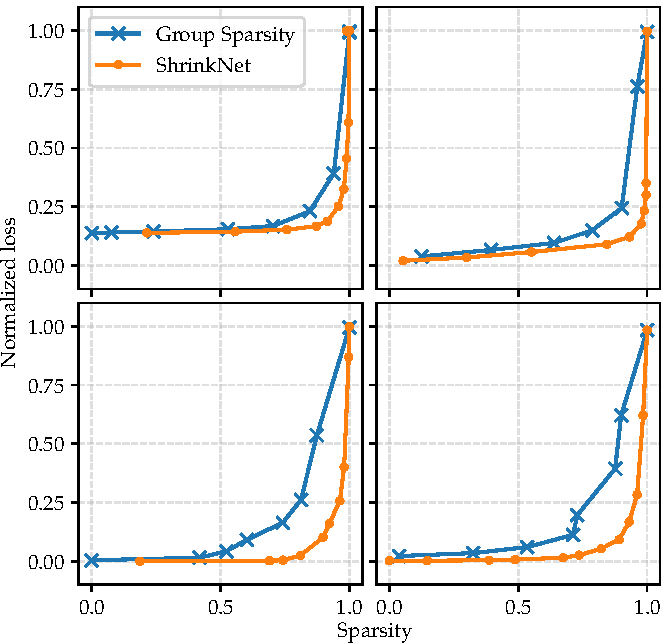
\includegraphics[width=\columnwidth]{regressions}
\vspace*{-5mm}
\caption{\label{sparsity_accuracy}Loss/Sparsity trade off comparison between Group Sparsity and Shrinknet on linear and logistic regression. From top to bottom and left to right we show the results for \texttt{scm1d}, \texttt{oes97}, \texttt{gina\_prior2} and \texttt{gsadd}.}

\end{center}
\vspace*{-4mm}
\end{figure}